\documentclass[crop]{standalone}
\usepackage[usenames,dvipsnames,svgnames]{xcolor}
\usepackage{tikz}
\usetikzlibrary{arrows,shapes} % tikz package already loaded by 'tikz' option
\makeatletter
\begin{document}
\newcommand{\dblue}    [1]	{\textcolor{RoyalBlue}{#1}}


%\tikzset{
%vertex/.style = {
%    circle,
%    fill            = black,
%    outer sep = 2pt,
%    inner sep = 1pt,
%}
%}
\hspace*{-.23cm}
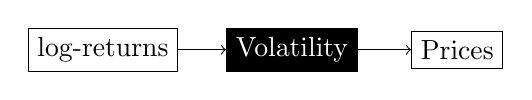
\begin{tikzpicture}
  
  % Opposition
  \node[draw] (A) {log-returns};
  \node[draw,fill=black,text=white] (B) at (2.4,0) {Volatility};
  \node[draw] (C) at (4.5,0) {Prices};
  \draw[->,draw] (A) to (B);
  \draw[->,draw] (B) to (C);
\end{tikzpicture}


\end{document}
